% Draft v0 (arXiv full version). Every line carrying a number ends with "% src: <file>:<line or table>".
% Paths are relative to the repository root. EXPL = exploration seeds (offset 0), VAL = validation (100), CONF = confirmatory (900000).
\documentclass[conference]{IEEEtran}
\usepackage{cite}
\usepackage{amsmath,amssymb}
\usepackage{graphicx}
\usepackage{booktabs}
\usepackage{url}
\usepackage{array}
\usepackage{microtype}

\newcommand{\POS}{\texttt{POS\_STEP}}
\newcommand{\TT}{\texttt{T2}}
\newcommand{\ATT}{\texttt{ATT\_STEP}}
\newcommand{\pp}{\,pp}
\newcommand{\estim}{\textsc{estim}}

\begin{document}

\title{Online Payload Estimation Nearly Closes the Centered Case but Not the Off-Center One in Docked Modular Multirotors}

\author{\IEEEauthorblockN{Hao-Ting Ho}
\IEEEauthorblockA{Department of Electrical Engineering, Tunghai University, Taichung, Taiwan\\
\texttt{haoting.ho@outlook.com}}}

\maketitle

\begin{abstract}
Several small quadrotor modules docked into one rigid body can be flown by a single centralized controller, but an unknown payload (mass and center-of-mass offset) invalidates the model that the controller's thrust allocation relies on.
We study this problem in a batched rigid-body simulator.
We build a ladder of classical controllers (QP thrust allocation, a yaw-rate limit, and recursive-least-squares payload estimation) and use a from-scratch PPO as a probe.
The pre-registration was frozen after the classical exploration runs and defines three disjoint seed sets; the classical results were then recomputed on the confirmatory set (the off-center scores had been seen before the freeze).
On exploration seeds, a 15\% payload costs the best classical baseline in that condition 14.4\% of its own nominal score, against 1.7\% for $\pm20\%$ thrust-coefficient error and 0.3\% for docking error. % src: results/p2/g2.md:27 (own-degradation column),30,31 (EXPL)
On confirmatory seeds with a centered payload, the estimator-equipped stack keeps 0.69--0.82 of its nominal score on the tracking task and 0.95--0.99 on the position step. % src: results/p2/classical_confirm.md:370,378,386,374,382,390
Its paired difference to a payload-informed reference is at most 0.007 (upper CI bound 0.019), within the point-mass payload model. % src: results/p2/classical_confirm.md:370,378,386,374,382,390,87,75,78,81,84,90 (largest paired difference +0.007, line8 POS_STEP, line 90)
For an off-center payload, a gap of 8/11/22\% (6/7/8 modules) remains in the position-step task. % src: README.md:24; results/p2/classical_confirm.md:281,285,289
A from-scratch PPO did not meet the pre-registered precondition for opening the main RL experiment within the recipe budget, and an exploratory residual PPO on top of the estimator stack did not close the remaining gap for two training seeds.
These RL statements hold for these recipes and this compute budget only.
\end{abstract}

\begin{IEEEkeywords}
modular aerial robots, payload estimation, thrust allocation, reinforcement learning, pre-registration
\end{IEEEkeywords}

\section{Introduction}
Small quadrotors can dock into a larger vehicle that flies as one rigid body~\cite{saldana2018modquad,xu2025modular,mu2020universal}.
Once docked, the thrust that each rotor must produce depends on the mass, inertia, and center of mass of the whole body.
A payload of unknown mass and position changes all three.

We study this problem for a single centralized controller.
We make no claim about decentralized control.
Three questions drive the paper.
(Q1) Which model error costs the most: payload, thrust-coefficient error, or docking error?
(Q2) How much of the payload cost can a classical stack that estimates the payload online recover, within the point-mass payload model?
(Q3) Can a learned controller whose actor cannot observe the payload close the gap that remains?

The main evidence is classical.
Reinforcement learning (RL) enters as a probe with a pre-registered stopping rule.
The main RL experiment would open only if a from-scratch policy on the six-module line reached 90\% of the estimator stack's tracking score under a 15\% payload. % src: docs/prereg.md:247,269
Development policies stayed below 90\% of B1 on at least one task even without a payload, so that test was never run. % src: README.md:66-71; results/p3/STATUS.md:121,128,159,160
The only RL result with a payload is an exploratory residual policy, and the negative outcome is reported as such.
The study was pre-registered (version 1.0, tag \texttt{prereg-v1.0}) with three disjoint seed sets, and the classical results were recomputed on fresh confirmatory seeds after the freeze. % src: docs/prereg.md:3,63-67,312,375
Contributions:
\begin{enumerate}
\item Classical result: on exploration seeds, payload is the costliest of the three model errors we compared; on confirmatory seeds, the estimator stack stays close to the informed reference for a centered payload and leaves a gap that grows with module count for an off-center payload (Sections~\ref{sec:classical} and~\ref{sec:results}).
\item RL result: the precondition of the pre-registered stopping rule was not met, so the main RL experiment was not opened, and an exploratory residual policy did not close the gap (Sections~\ref{sec:rl} and~\ref{sec:results}).
\item A protocol record: what was frozen, what was chosen after seeing classical results, what was never run, and one erratum (Section~\ref{sec:protocol}).
\end{enumerate}
Non-claims: there is no hardware experiment; the payload is a point mass; the E3 condition lies at a corner of the training range and is not out-of-distribution; and no test of ``RL versus classical'' was run.
Code and logs: \url{https://github.com/Jadiouo/docked-multirotor-payload}.

\section{Related Work}
Prior work on modular vehicles covers assembly, control, and configuration estimation.
ModQuad demonstrated quadrotor modules that self-assemble in flight~\cite{saldana2018modquad}.
Later work extends the control of docked modules~\cite{xu2025modular}, adds model-predictive control with a thrust allocator~\cite{huang2026mars}, and plans self-reconfiguration without learning~\cite{huang2025transformars}.
UFO estimates the configuration of a modular multirotor from several IMUs and refines it with an adaptive geometric controller~\cite{mu2020universal}.
In our reading of that paper, it needs an identification phase with hand rotation and assumes parallel thrust directions and a plate payload.
Our estimator runs online from the first step with no identification phase, but it assumes a point-mass payload.

The closest learning work conditions one policy on the allocation matrix for fixed-motor-count families, whereas we study a docked rigid body with a payload and compare against classical estimation.
That work trains one PPO policy with recurrent memory for quadrotor and hexarotor families~\cite{konstantaropoulos2026embodiment}.
Other work adapts one policy across quadrotor scales or morphologies~\cite{vaidya2025dynamics,eschmann2025raptor,rehberg2026efficient}.
The graph-style policy in our probe follows morphology-general RL from locomotion~\cite{huang2020one,engwegen2025shared,luo2025gcnt}.
RL has been used for the docking maneuver of two vehicles~\cite{feng2024enhancing}.
To our knowledge, as of a literature search in October 2026, no work uses RL to control the already-docked rigid structure.

Our classical baselines build on adaptive control, in which INDI handles model error through measured angular acceleration~\cite{smeur2016adaptive,smeur2018cascaded,sun2020incremental}.
Recursive least-squares estimation of control effectiveness has been used on single quadrotors~\cite{blaha2024control,blaha2024flying}.
We include an INDI baseline and build the estimator on the same idea of regression on thrust.

\section{System and Tasks}\label{sec:system}
The simulator integrates a single rigid body for all modules in a batch.
The physical step is 0.002~s and the controller runs at 100~Hz; each motor follows a first-order lag with time constant 0.07~s; gyroscope and accelerometer noise have standard deviations 0.01~rad/s and 0.05~m/s$^2$. % src: docs/env_spec.md:13,15,47
Docked modules form one body with no contact or joint dynamics; a crash is declared when height falls below zero, position error exceeds 3~m, or tilt exceeds 100$^\circ$. % src: docs/env_spec.md:4,60
Episodes last 5~s. % src: docs/env_spec.md:59
Module mass, inertia, and spacing come from a CAD model of the module (\texttt{cad/}). % src: docs/env_spec.md:12
Configuration \emph{line-$N$} is $N$ modules in a row; we use $N=6,7,8$; \emph{grid10} is 10 modules in a $5\times2$ grid (5 along $x$, 2 along $y$), used only in the mid-flight event study. % src: quadsim/assembly.py:21,22,24,29; docs/prereg.md:161
Fig.~\ref{fig:overview} shows the top view of line-6, line-7 and line-8 and the payload attach points of E1 and E3. % src: quadsim/assembly.py:21,22,29,35-52; quadsim/module_params.py:24; cad/out/module_props.json:pitch; docs/prereg.md:170,177
\begin{figure*}[!t]
\centering
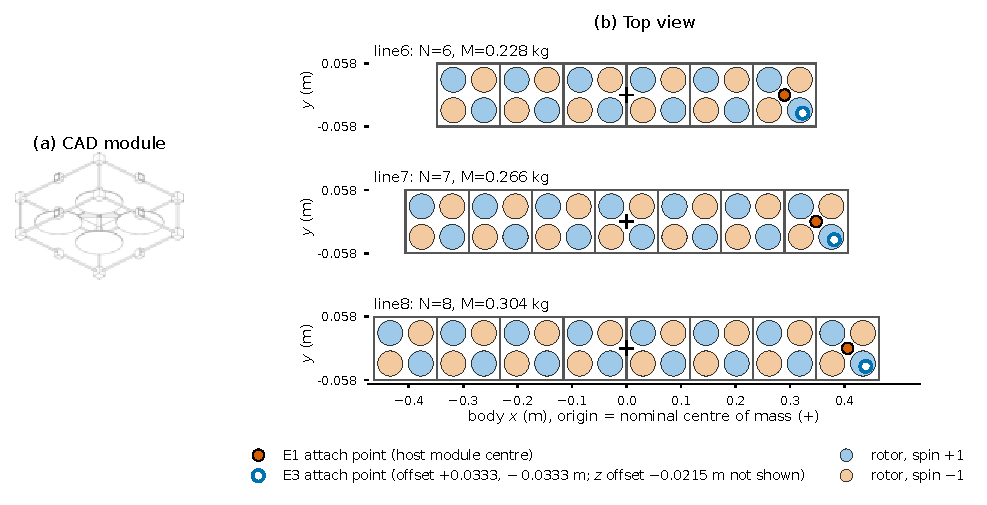
\includegraphics[width=0.78\textwidth]{figs/fig1_overview.pdf}
\caption{System overview. (a) CAD model of one module. (b) Top view of line6, line7 and line8 in the body frame (x forward, y left), module pitch 0.116~m, rotor radius 0.023~m, each module with four rotors at $(\pm0.028,\pm0.028)$~m from its center; the origin (+) is the nominal center of mass (without payload). Filled marker: E1 payload attach point at the center of the module with largest $x$. Open marker: E3 attach point, offset $(+0.0333,-0.0333)$~m in the $x$--$y$ plane; the $z$ offset of $-0.0215$~m is not visible in this view.}\label{fig:overview}% src: paper/figs/captions.md:5; quadsim/params.py:4-8; cad/out/module_props.json:pitch,prop_radius_m; docs/prereg.md:177
\end{figure*}

We evaluate three tasks with one score.
\TT\ (the tracking task) tracks a set point that changes every 1.5~s (position within $\pm1$~m, yaw within $\pm90^\circ$). % src: docs/env_spec.md:55
\POS\ (the position step) is a 1.5~m position step and \ATT\ a 0.8--1.2~rad attitude step; \emph{HOVER} is \POS\ with a zero step, so the payload event happens during hover (event study only). % src: docs/env_spec.md:57,58; scripts/rqd_classical.py:5,114-115
The score of an episode is $\text{success}\times\max(0,\,1-e_\mathrm{rms}/e_\mathrm{ref})$, with $e_\mathrm{ref}=1.0$~rad for \ATT\ and 1.5~m for \POS\ and \TT. % src: docs/prereg.md:54
A score of 1 is perfect and 0 is a crash or no correction.
A recovery task, used only for RL training, starts from a random attitude and returns to hover. % src: docs/env_spec.md:54
Each cell uses 100 episodes. % src: docs/prereg.md:56

The payload is a point mass attached at a module center or at a fixed offset; its mass is a fraction of the total mass. % src: docs/env_spec.md:70; quadsim/controllers.py:999
The conditions used here are:
\begin{itemize}
\item \textbf{E1}: a 15\% payload on the module with largest $x$, no offset, present from $t=0$. % src: docs/prereg.md:170
\item \textbf{E3}: E1 plus an offset of $(+0.0333,-0.0333,-0.0215)$~m, a corner of the training range of the offset (so not out-of-distribution). % src: docs/prereg.md:177,314
\item \textbf{Event}: the payload is attached or dropped mid-flight, at a module center or off-center.
\item \textbf{Nominal}: no payload.
\end{itemize}
A 15\% payload is feasible for hover at a thrust-to-weight ratio of 1.36; a 30\% payload is infeasible at 1.12 on all six configurations tested, so payload studies stay at 10--15\%; residual-RL training randomizes the payload up to 20\%. % src: results/p2/g2.md:13-18; results/p3/res_line6_off_k2_h4/args.json (payload_max 0.2)

This comparison favors the classical controllers.
They read true position, velocity, attitude, and angular rate, and the leader knows the nominal shape; the RL actor sees true position, velocity, and attitude but a noisy gyroscope and accelerometer, and only $k$-hop shape information. % src: docs/prereg.md:41-44,46
A variant of the classical stack with noisy angular rate (called A3 in the pre-registration) was specified but not run. % src: docs/prereg.md:235,325

\section{Classical Controller Ladder}\label{sec:classical}
All classical controllers share one outer loop: a position PD law produces a desired acceleration, from which a geometric attitude law produces an angular-acceleration command; the gains are normalized by mass and inertia, so one set serves all configurations. % src: quadsim/controllers.py:3-9
They differ in the allocation layer and in what they know about the payload.
\begin{itemize}
\item \textbf{B1}: the leader knows the nominal shape and allocates by pseudoinverse and clipping. % src: quadsim/controllers.py:153
\item \textbf{B1-QP}: the same wrench, allocated by bounded least squares; under saturation roll and pitch have priority over thrust, and thrust over yaw. % src: quadsim/controllers.py:170-175
\item \textbf{yawlim}: the yaw reference follows the target at a bounded rate $\mathrm{rate}_c\sqrt{\alpha_{\mathrm{yaw}}}$, where $\alpha_{\mathrm{yaw}}$ is the nominal yaw angular-acceleration authority of the configuration. We use $\mathrm{rate}_c=0.556$, selected from 20 settings on training configurations. % src: quadsim/controllers.py:506-510; docs/prereg.md:139
\item \textbf{estim}: payload estimation by recursive least squares with forgetting. Total mass is estimated by regressing accelerometer specific force on summed thrust; the center-of-mass offset is estimated by regressing the torque residual on summed thrust. The payload is then treated as a point mass to rebuild the center of mass, inertia, and allocation matrix. The estimator uses only the noisy gyroscope and accelerometer and the controller's own motor commands. % src: results/p2/g2_estim.md:5
\item \textbf{estim-reset}: \textbf{estim} plus a CUSUM change detector that resets the regression after a mid-flight event. % src: quadsim/controllers.py:1018-1022
\item \textbf{B3 INDI} and \textbf{B3+adapt}: incremental dynamic inversion, without and with a per-axis gain adaptation. % src: quadsim/controllers.py:640-642
\item \textbf{informed} controllers (called the informed reference in the text) are given the true payload model and allocate with it. \textbf{informed-offset} also knows the offset; \textbf{informed-event} also knows the event. % src: docs/prereg.md:142
\end{itemize}
The main configuration is \textbf{B1-QP-estim-yawlim} (\textbf{estim-yawlim} below).
Its optional snap step projects the center-of-mass estimate to the nearest module center; the main configuration has snap off.

The informed controllers are references, not upper bounds.
Their angular-acceleration limits remain nominal, and in conditions with thrust-coefficient and docking errors they do not know those errors. % src: docs/prereg.md:333
A controller outside this family could score higher.

The classical side had 20 settings each for the estimator, yawlim, and reset detector (60 in total). % src: docs/prereg.md:338
The estimator and detector settings were scored on 32 validation episodes per setting; yawlim was tuned on training configurations. % src: docs/prereg.md:338,139
The estimator settings were selected with snap on and a payload at a module center, and then run with snap off and no retuning. % src: results/p2/g2_estim.md:7,114; results/p2/classical_confirm.md:4; README.md:69
All confirmatory results use the same settings, without retuning. % src: results/p2/classical_confirm.md:4

\section{Reinforcement-Learning Probe}\label{sec:rl}
The probe uses a PPO~\cite{schulman2017proximal} written from scratch (\texttt{ppo.py}); Appendix~\ref{app:hopper} compares it with CleanRL~\cite{huang2022cleanrl}.
The policy is a graph network over modules with $k=2$ hops of neighbor information and a history of $H=4$ steps; training uses 512 environments per (configuration, task) pair (1024 for the two-task runs here) and hidden width 64. % src: results/p3/line6_nom_k2_h4/args.json:3-6,8-9,14,15,16; results/p3/res_line6_off_k2_h4/args.json:3-7,8-10; scripts/rl_train.py:91-92 (a single n-envs value is repeated per spec)
The actor outputs a normalized command per motor. % src: docs/env_spec.md:49-51
It cannot observe the payload.
The critic receives four privileged payload fields during training only. % src: docs/prereg.md:40
The base recipe trains on line6 with a recovery task (\texttt{T1}) and the \TT\ task for $1.5\times10^8$ steps from training seed 7. % src: results/p3/line6_nom_k2_h4/args.json:3-5,12,32

The pre-registration allowed at most two recipe changes after the base recipe. % src: docs/prereg.md:339
We tried (i) a penalty on action means outside the bounds (mean-bound, $4\times10^7$ steps), and (ii) one sample per team with the same penalty ($1.5\times10^8$ steps). % src: results/p3/STATUS.md:118,126
If line6 did not meet the pre-registered precondition after the budget, the main RL experiment would not be opened (prereg.\ rule 7.3(b)). % src: docs/prereg.md:264,373

Because the main experiment was not opened, we trained a residual policy: $u=\mathrm{clip}(u_{\estim\text{-}yawlim}+0.2\,\delta)$. % src: docs/prereg.md:369; results/p3/STATUS.md:133
It trains on line6 \TT\ and \POS\ with payloads up to 20\% and random offsets, stopped by a 120-minute cap after $3.27\times10^7$ steps (1000 of 1831 planned iterations). % src: results/p3/STATUS.md:133; results/p3/res_line6_off_k2_h4/args.json:4-5,28,34
It was evaluated on validation and exploration seeds only and never on confirmatory seeds. % src: docs/prereg.md:370

Most recipes have a single development seed; seed 8 was added for the mean-bound and residual recipes after the freeze. % src: README.md:137; docs/prereg.md:376
All RL conclusions below are exploratory.

\section{Protocol}\label{sec:protocol}
Pre-registration v1.0 was frozen on 2026-11-01 under the tag \texttt{prereg-v1.0}, before any RL policy was evaluated on confirmatory seeds; in the end none was. % src: docs/prereg.md:3,373
The tag was first placed on an unfinished commit and moved a few minutes later, before any confirmatory result existed. % src: docs/prereg.md:352
Three seed sets, with environment seeds disjoint by construction, are used as in Table~\ref{tab:seeds}. % src: docs/prereg.md:63-67
Training environment seeds ($\text{seed}\times1000+i$) lie outside all three sets. The formal training seeds 101--112 were never used; the development runs use seeds 7 and 8. % src: docs/prereg.md:78,85,373,376

\begin{table}[t]
\caption{Seed sets (environment-seed offsets).}\label{tab:seeds}
\centering\small
\begin{tabular}{@{}llp{4.6cm}@{}}
\toprule
Set & Offset & Use \\
\midrule
Exploration & 0 & classical diagnostics; early RL numbers \\ % src: docs/prereg.md:66
Validation & 100 & tuning of the estimator; RL evaluation reported here, except the four-configuration run (offset 0) \\ % src: docs/prereg.md:65; results/p2/g2_estim.md:9; results/p3/train4_mix_k1_h4/eval_final.json (no seed_offset, i.e. offset 0)
Confirmatory & 900000 & classical recomputation after the freeze \\ % src: docs/prereg.md:67,375
\bottomrule
\end{tabular}
\end{table}

Two choices were made after the classical exploration results were known, and before any RL evaluation.
First, snap off as the main setting was chosen after diagnostics showed that snap on fails for off-center payloads. % src: docs/prereg.md:147
Second, the E3 cell was chosen after the classical gap decomposition. % src: docs/prereg.md:178
In addition, the main E3 task was switched from \TT\ to \POS\ by a rule written in advance (largest mean relative gap on exploration seeds); the switch was made before any RL evaluation on E3. % src: docs/prereg.md:180,351
Confirmatory E3 scores had already been computed before the freeze and entered in the pre-registration, so E3 is not a blind confirmation. % src: docs/prereg.md:375; results/p2/classical_confirm.md:317-332

None of the pre-registered hypothesis tests was run. The pre-registration specified equivalence tests on E1 (two one-sided $t$ intervals over training seeds) and one-sided superiority tests on E3 \POS\ with Holm correction~\cite{holm1979simple}. % src: docs/prereg.md:90-92,98-100,107-113
They compare the trained RL policy with estim-yawlim over formal training seeds, and the main RL experiment that would supply those seeds was not opened (rule 7.3(b)).
The formal precondition evaluation (training seed 101) was also never run; the decision rested on the development runs. % src: docs/prereg.md:350,373
We therefore wrote the RL outcome as ``did not meet the pre-registered precondition for opening the main RL experiment within the recipe budget,'' not as a failed test.
No RL-versus-classical hypothesis test is reported.

After the freeze we recomputed the classical results on confirmatory seeds: 384 cells, no retuning. % src: docs/prereg.md:375; results/p2/classical_confirm.md:4; results/p2/classical_confirm_raw.json (384 keys: E1 54, E2 90, E3 24, NOM 24, EV 192; counted)
All directions agree with exploration seeds. % src: docs/prereg.md:375
A mechanical rule flagged 9 comparison rows as inconsistent; in all nine the exploration--confirmatory difference is within $\pm0.015$ and the confirmatory paired difference is at most 0.006, so no conclusion flips (rows listed in \texttt{results/p2/classical\_confirm.md}). % src: results/p2/classical_confirm.md:87,283,287,593,638,671,683,710,719; README.md:29
Confirmatory \TT\ scores run about 0.02--0.05 above exploration scores. % src: README.md:31
Intervals are 95\% percentile bootstrap intervals over episodes (2000 resamples)~\cite{efron1993introduction}; paired differences are bootstrapped per episode. % src: results/p2/classical_confirm.md:5
They are conditional on the fixed set of 100 episodes and do not cover the choice of that set. % src: results/p2/classical_confirm.md:5; README.md:137
One erratum: the pre-registration text said that 6 of 12 cells of the multi-configuration RL run were below 0.90 of B1; the correct count is 4. % src: docs/prereg.md:353; results/p3/STATUS.md:86
A second slip, a swapped snap-on/snap-off order in one table, was corrected on 2026-10-31 and does not change a conclusion. % src: results/p2/p3d_factorial.md:8

\section{Results}\label{sec:results}
\subsection{Payload is the costliest of the three model errors compared (exploration seeds only)}
Over five configurations and two tasks, the best nominal classical baseline (B1-QP) scores 0.497. % src: results/p2/g2.md:22
With a 15\% payload, the best classical baseline under payload (INDI) loses 14.4\% of its own nominal score, and B1-QP loses 90.4\% of its own. % src: results/p2/g2.md:27 (columns ``own degradation'': 14.4 and 90.4)
A $\pm20\%$ thrust-coefficient error costs the best baseline 1.7\%, and $\pm5$~mm, $\pm2^\circ$ docking error costs 0.3\% (both B1-QP, each relative to its own nominal score). % src: results/p2/g2.md:30,31
These numbers use exploration seeds and were not recomputed on confirmatory seeds. % src: README.md:32
We therefore treat payload as the main error in the rest of the paper.

\subsection{With a centered payload, estim-yawlim stays close to the informed reference (confirmatory)}
Table~\ref{tab:classical} and Fig.~\ref{fig:classical}(a) give the E1 results.
\begin{figure*}[!t]
\centering
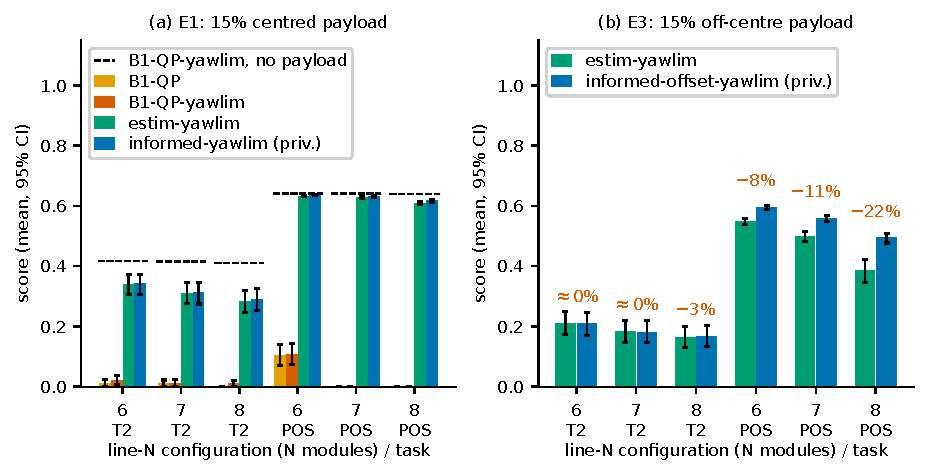
\includegraphics[width=0.78\textwidth]{figs/fig2_classical.pdf}
\caption{estim-yawlim tracks the informed reference closely in all cells except the off-center position step, where the gap grows with module count. Classical results on confirmatory seeds (seed offset 900000, 100 episodes per cell). Informed is informed-yawlim in (a) and informed-offset-yawlim in (b). (a) E1, centered 15\% payload. (b) E3, off-center 15\% payload. Percentages in (b): gap of estim-yawlim relative to informed-offset-yawlim, (inf$-$est)/inf, from the plotted means ($\approx$0\%: below 0.5\%). Dashed: B1-QP-yawlim without payload (same seeds). Error bars: 95\% bootstrap CI over episodes. \TT\ differences between estim-yawlim and informed lie within the 95\% CIs. POS = \POS.}\label{fig:classical}% src: paper/figs/captions.md:9-10
\end{figure*}
Without payload knowledge, B1-QP-yawlim collapses on \TT: 0.021, 0.011, 0.009 on line6/7/8, with success 11\%, 6\%, 3\%. % src: results/p2/classical_confirm.md:18,36,54
The INDI baseline reaches 0.224, 0.181, 0.155 on \TT. % src: results/p2/classical_confirm.md:19,37,55
estim-yawlim scores 0.340, 0.310, 0.283, and the informed reference scores 0.341, 0.311, 0.289. % src: results/p2/classical_confirm.md:24,42,60,22,40,58
The paired difference informed minus estim on \TT\ is $+0.001$, $+0.001$, $+0.006$, and all three 95\% intervals contain 0. % src: results/p2/classical_confirm.md:75,81,87
On \POS\ the paired differences are $+0.002$, $+0.003$, $+0.007$, and the intervals exclude 0 but are small. % src: results/p2/classical_confirm.md:78,84,90
Within the point-mass payload model, estim-yawlim therefore reaches the informed reference to within 0.007 on E1; no equivalence test was run, and the widest interval (line8 \TT) has upper bound $+0.019$, about 7\% of the reference score. % src: results/p2/classical_confirm.md:87
Relative to its own no-payload score (not listed in Table~\ref{tab:classical}), estim-yawlim keeps 0.815, 0.748, 0.689 on \TT\ and 0.987, 0.978, 0.953 on \POS. % src: results/p2/classical_confirm.md:370,378,386,374,382,390 (ratio to estim-yawlim's own nominal, e.g. line 374: 0.633/0.641=0.987)
The loss on \TT\ grows with the number of modules.
The reference shows the same pattern (0.341, 0.311, 0.289 against a nominal 0.417, 0.415, 0.411).
We read this as a physical limit and not an estimation limit (our interpretation; the pre-registration says the same for exploration snap-on numbers). % src: results/p2/classical_confirm.md:22,40,58,340,348,356; docs/prereg.md:33

yawlim itself matters on the nominal task: on line8 \TT, B1-QP scores 0.328 (success 87\%) and B1-QP-yawlim 0.411 (100\%). % src: results/p2/classical_confirm.md:355,356

\begin{table*}[t]
\caption{With a centered payload estim-yawlim stays close to the informed reference; with an off-center payload it falls short on the position step, more so with more modules. Classical results on confirmatory seeds (offset 900000, 100 episodes per cell). Scores are means; ``informed'' is the informed reference (informed-yawlim for E1, informed-offset-yawlim for E3), not an upper bound. The last column is informed $-$ estim (paired, 95\% bootstrap CI). Gap is (informed $-$ estim)/informed for E3 \POS. The ``No payload'' column is B1-QP-yawlim without payload; the B1-QP-yawlim column is with the payload of the row's condition.}\label{tab:classical} % src: docs/prereg.md:56,67
\centering\small
\begin{tabular}{@{}llcccccc@{}}
\toprule
Cond. & Task, config & No payload & B1-QP-yawlim & estim-yawlim & informed & informed $-$ estim [95\% CI] & Gap \\
\midrule
E1 & \TT, line6 & 0.417 & 0.021 & 0.340 & 0.341 & $+0.001$ [$-0.001$, $+0.003$] & -- \\ % src: classical_confirm.md:340,18,24,22,75
E1 & \TT, line7 & 0.415 & 0.011 & 0.310 & 0.311 & $+0.001$ [$-0.006$, $+0.005$] & -- \\ % src: classical_confirm.md:348,36,42,40,81
E1 & \TT, line8 & 0.411 & 0.009 & 0.283 & 0.289 & $+0.006$ [$-0.005$, $+0.019$] & -- \\ % src: classical_confirm.md:356,54,60,58,87
E1 & \POS, line6 & 0.642 & 0.107 & 0.633 & 0.635 & $+0.002$ [$+0.002$, $+0.003$] & -- \\ % src: classical_confirm.md:344,27,33,31,78
E1 & \POS, line7 & 0.642 & 0.000 & 0.628 & 0.631 & $+0.003$ [$+0.003$, $+0.004$] & -- \\ % src: classical_confirm.md:352,45,51,49,84
E1 & \POS, line8 & 0.640 & 0.000 & 0.610 & 0.616 & $+0.007$ [$+0.006$, $+0.008$] & -- \\ % src: classical_confirm.md:360,63,69,67,90
\midrule
E3 & \TT, line6 & 0.417 & 0.000 & 0.210 & 0.209 & $-0.001$ [$-0.008$, $+0.006$] & -- \\ % src: classical_confirm.md:340,257,258,259,283
E3 & \TT, line7 & 0.415 & 0.000 & 0.182 & 0.181 & $-0.001$ [$-0.010$, $+0.007$] & -- \\ % src: classical_confirm.md:348,265,266,267,287
E3 & \TT, line8 & 0.411 & 0.000 & 0.163 & 0.168 & $+0.005$ [$-0.007$, $+0.016$] & -- \\ % src: classical_confirm.md:356,273,274,275,291
E3 & \POS, line6 & 0.642 & 0.000 & 0.548 & 0.595 & $+0.047$ [$+0.041$, $+0.052$] & 8\% \\ % src: classical_confirm.md:344,253,254,255,281; README.md:24
E3 & \POS, line7 & 0.642 & 0.000 & 0.498 & 0.559 & $+0.061$ [$+0.052$, $+0.070$] & 11\% \\ % src: classical_confirm.md:352,261,262,263,285; README.md:24
E3 & \POS, line8 & 0.640 & 0.000 & 0.385 & 0.494 & $+0.108$ [$+0.084$, $+0.134$] & 22\% \\ % src: classical_confirm.md:360,269,270,271,289; README.md:24
\bottomrule
\end{tabular}
\end{table*}

\subsection{With an off-center payload, a gap remains in the position step (confirmatory)}
With an off-center payload, B1-QP and B1-QP-yawlim score 0 on every cell. % src: results/p2/classical_confirm.md:252-253,256-257,260-261,264-265,268-269,272-273
On \TT\ estim-yawlim and the informed reference differ by at most 0.005 in score, and all three intervals contain 0. % src: results/p2/classical_confirm.md:283,287,291
On \POS\ a gap remains: informed minus estim is $+0.047$, $+0.061$, $+0.108$ for line6/7/8, with 95\% intervals that exclude 0. % src: results/p2/classical_confirm.md:281,285,289
Relative to the informed score (0.595, 0.559, 0.494) this is 8\%, 11\%, 22\%; computed from the table values it is 7.9\%, 10.9\%, 21.9\%. % src: README.md:24; results/p2/classical_confirm.md:255,263,271 (derived: 0.047/0.595, 0.061/0.559, 0.108/0.494)
We use this denominator throughout.
The same \POS\ data give informed/estim ratios of 1.086, 1.123, 1.281. % src: results/p2/classical_confirm.md:281,285,289

On exploration seeds a factorial analysis helps to locate the gap (not recomputed on confirmatory seeds).
Here the gap is the percent shortfall relative to the informed reference, pooled over the six E3 cells (three configurations, two tasks). % src: results/p2/p3d_resolve.md:3,11 (EXPL)
Starting the payload at $t=0$ instead of attaching it later reduces the gap by 6.7\pp, and a random instead of farthest mount reduces it by 6.0\pp; the estimator version reduces it by 0\pp.
The source marks the mechanism as inference, and we have not isolated it.

With an off-center payload, the estim-yawlim stack with snap on scored 0.000 on line6 and line8 \TT, against 0.197 and 0.131 with snap off (success 0\% versus 74\% and 58\%; exploration seeds). % src: results/p2/p3d_factorial.md:8 (EXPL)
With the payload at a module center the two settings differ by at most 0.002. % src: results/p2/p3d_factorial.md:8
The estimator was tuned and evaluated only with centered payloads, so the failure was not visible during tuning. % src: README.md:69

\subsection{After mid-flight payload events, the reset estimator recovers the informed reference on average (confirmatory)}
We compare estim-yawlim with and without the change-point reset against the informed reference that knows the event, averaged over four configurations (line6, line7, line8, grid10) and three tasks. % src: docs/prereg.md:161; paper/figs/rqd_aggregate.csv
With the reset, the estimator reaches 0.98--1.00 of the informed reference's score in all twelve task-by-condition rows. % src: paper/figs/rqd_aggregate.csv:col ratio_estim_reset_yawlim (min 0.9785, max 0.9994); docs/prereg.md:375
Without the reset, it reaches 0.89--0.98 for centered events and 0.67--0.89 for off-center events. % src: paper/figs/rqd_aggregate.csv:col ratio_estim_yawlim (centered 0.8939--0.9790; off-center 0.6709--0.8931)
Within the point-mass model, the reset estimator thus recovers the informed reference on average.
Per-configuration rows are in \texttt{results/p2/classical\_confirm.md} (the EV section); the aggregate is computed in \texttt{paper/figs/rqd\_aggregate.csv}. % src: results/p2/classical_confirm.md:392-588

\subsection{RL neither met the precondition nor closed the gap (validation seeds, exploratory)}
Table~\ref{tab:rl} and Fig.~\ref{fig:rl} give the RL results.
\begin{table*}[!t]
\caption{Every from-scratch recipe fell below 90\% of B1 on at least one no-payload task, and the residual policy did not improve on estim-yawlim. RL probe on validation seeds (offset 100, 100 episodes per cell; exploratory; final checkpoint). (a) From scratch on line6 without payload, as a ratio of the RL score to the denominator named in the last column. ``B1'' means the score of B1; ``max'' means max(B1, B1-QP). (b) Residual RL on line6 E3, absolute scores; the residual is added to estim-yawlim, the classical estimator stack.}\label{tab:rl} % src: docs/prereg.md:56,65,103
\centering\small
\begin{tabular}{@{}llcccl@{}}
\toprule
\multicolumn{6}{@{}l}{(a) From scratch, line6 nominal: RL score / denominator} \\
Recipe & Train seed & \ATT & \POS & \TT & Denominator \\
\midrule
Base & 7 & 0.61 & 0.70 & 0.79 & B1 \\ % src: README.md:74
Base & 7 & 0.606 & 0.701 & 0.745 & max \\ % src: results/p3/STATUS.md:112-114
Mean-bound & 7 & 0.491 & 0.892 & 0.929 & B1 \\ % src: results/p3/STATUS.md:121,159
Mean-bound & 8 & 0.634 & 0.707 & 0.661 & B1 \\ % src: results/p3/STATUS.md:160
Team-sample & 7 & 0.759 & 0.405 & 0.626 & B1 \\ % src: results/p3/STATUS.md:128
\midrule
\multicolumn{6}{@{}l}{Pipeline check, single module (not line6; one policy, seed 0): ratio to max} \\ % src: README.md:137
Single-module mix & 0 & 1.046 & 1.054 & 1.099 & max \\ % src: results/p3/STATUS.md:103-105
\midrule
\multicolumn{6}{@{}l}{(b) Residual RL, line6 E3: absolute score} \\
 & & \ATT & \POS & \TT & \\
\midrule
Residual & 7 & 0.353 & 0.554 & 0.225 & -- \\ % src: results/p3/STATUS.md:140,154
Residual & 8 & 0.353 & 0.555 & 0.224 & -- \\ % src: results/p3/STATUS.md:155
estim-yawlim & -- & 0.354 & 0.565 & 0.239 & -- \\ % src: results/p3/STATUS.md:140
informed reference & -- & 0.358 & 0.604 & 0.245 & -- \\ % src: results/p3/STATUS.md:140
\bottomrule
\end{tabular}
\end{table*}

\begin{figure*}[!t]
\centering
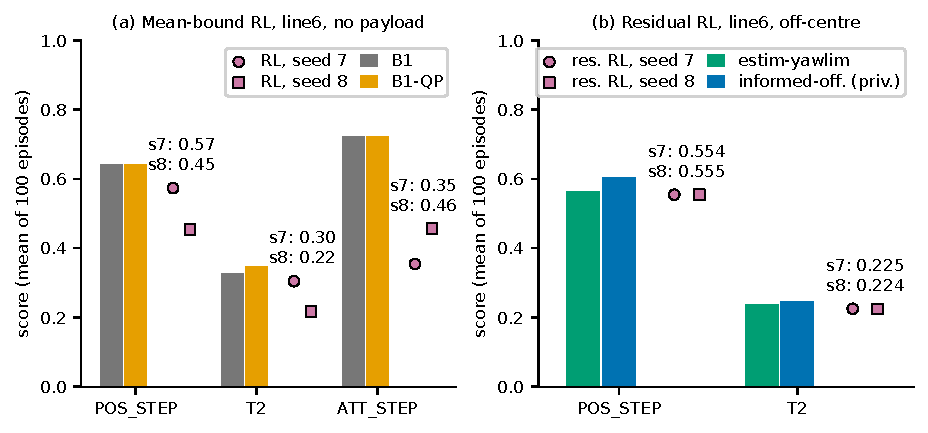
\includegraphics[width=0.78\textwidth]{figs/fig3_rl_probe.pdf}
\caption{Mean-bound RL stays below B1 on every no-payload task, and the residual policy stays slightly below estim-yawlim under an off-center payload. RL probe on validation seeds (seed offset 100, 100 episodes per cell); exploratory. (a) Mean-bound RL on line6 without payload; (b) residual RL on line6 with off-center payload (E3). Circle = RL training seed 7, square = RL training seed 8; label = seed 7/seed 8. Bars: classical controllers evaluated on the same validation episodes. Error bars: none (the RL/validation JSON files store only per-cell means, no per-episode scores or CI). Not comparable with Fig.~\ref{fig:classical} (different seed group).}\label{fig:rl}% src: paper/figs/captions.md:14-15
\end{figure*}
All RL numbers use validation seeds, 100 episodes per cell, and the final checkpoint, except the four-configuration run, which used exploration seeds (offset 0); all are exploratory. % src: results/p3/STATUS.md:109,145-146; docs/prereg.md:103; results/p3/train4_mix_k1_h4/eval_final.json (no seed_offset)
RL scores are not comparable with the confirmatory numbers of Table~\ref{tab:classical} because the seed sets differ. % src: paper/figs/captions.md:15; docs/prereg.md:65

From scratch on line6 without payload, the base recipe reaches 0.61, 0.70, 0.79 of B1 on \ATT, \POS, \TT. % src: README.md:74
Against the stronger of B1 and B1-QP, written max(B1, B1-QP), the same run gives 0.606, 0.701, 0.745. % src: results/p3/STATUS.md:112-114
Its training success rate fell during training (\TT\ from 0.61 to 0.45). % src: results/p3/STATUS.md:115
The RL policy saturated its actions in 0.490 of steps on line6 \TT, against 0.149 for B1 and 0.170 for B1-QP. % src: results/p3/STATUS.md:119
The recorded failure mode is tilt flip. % src: README.md:78
The mean-bound penalty reduced saturation to 0.157 but did not improve all tasks: ratios of 0.491, 0.892, 0.929 for seed 7 and 0.634, 0.707, 0.661 for seed 8. % src: results/p3/STATUS.md:120,159,160
The mean-bound run also used a different learning-rate schedule than the base run, so the comparison is not controlled. % src: results/p3/STATUS.md:122
The team-sample recipe gives 0.759, 0.405, 0.626, and the recipe budget is used up. % src: results/p3/STATUS.md:128,129
Every recipe left at least one no-payload task below $0.90\times$B1 (Table~\ref{tab:rl}), so we judged the precondition for the main experiment unmet. % src: Table~\ref{tab:rl}

As a pipeline check, a single-module policy trained on the same code reaches 1.046, 1.054, 1.099 of max(B1, B1-QP) with 100\% success. % src: results/p3/STATUS.md:103-105
A policy trained jointly on four configurations plateaued, with 4 of 12 cells below 0.90 of B1 (exploration seeds). % src: results/p3/STATUS.md:86; docs/prereg.md:262
We report this as a sanity check only; the multi-configuration problem is unsolved here.

On line6 E3 \POS, the residual policy scores 0.554 (seed 7) and 0.555 (seed 8), against 0.565 for estim-yawlim and 0.604 for the informed reference. % src: results/p3/STATUS.md:140,154,155
The paired differences against estim-yawlim are $-0.010$ [$-0.013$, $-0.008$] and $-0.010$ [$-0.011$, $-0.009$]. % src: results/p3/STATUS.md:154,155
On E3 \TT\ it scores 0.225 and 0.224, against 0.239 and 0.245. % src: results/p3/STATUS.md:140,154,155 (T2 column); paper/figs/fig3_rl_probe.png
The two seeds differ by at most 0.002 on every cell, and each seed was trained once. % src: results/p3/STATUS.md:162
The residual did not close the gap: it is slightly below estim-yawlim on both seeds, and two seeds that agree to within 0.002 are consistent with a correction close to zero (its magnitude was not measured).
Nominal-condition \TT\ for the residual is 1.27 of B1, but the evaluation did not list nominal estim-yawlim, so we do not credit the residual for it. % src: results/p3/STATUS.md:142


\section{Limitations}
Each item names the conclusion it limits and what the reader should not infer.
\begin{itemize}
\item \emph{Two development seeds for RL.} Most recipes were trained with one development seed, and only the mean-bound and residual recipes with a second (seed 8). We consider one or two seeds too few for a conclusion about RL, and the two mean-bound seeds disagree strongly (\TT\ ratio 0.929 and 0.661). The RL results show only that these one- or two-seed runs, these recipes, and this compute budget did not close the gap; they do not show that RL cannot. The residual runs also hit the time cap, and the mean-bound recipe differs from the base in learning-rate schedule. % src: README.md:137; results/p3/STATUS.md:122,133,159,160
\item \emph{Pre-registration frozen after classical exploration.} Snap off and the E3 cell were chosen after the classical results were seen, and the confirmatory E3 scores were seen before the freeze (Section~\ref{sec:protocol}). The E3 result is therefore not a blind confirmation, and E3 was chosen knowing where the exploration gap appeared.
\item \emph{Simulation and a point-mass payload.} There is no hardware, and the estimator and the environment share the point-mass payload model, so ``recovers'' holds only within that model. Off-center payloads and snap off test the circularity only in part, and the results do not transfer to hardware or to non-point-mass, flexible, or jointed payloads. % src: README.md:133,135; docs/prereg.md:31-32
\item \emph{Estimator tuned on centered payloads only.} The estimator was tuned only with centered payloads, and we did not test retuning on off-center payloads, so the off-center result applies to the estimator as tuned. % src: README.md:69
\item \emph{Tuning and information favor the classical side.} The classical stack reads true state and the full nominal shape, while the RL actor sees a noisy gyroscope and accelerometer and only $k$-hop shape information (Section~\ref{sec:system}); the noisy-rate variant A3 was not run. The classical gains and settings were tuned on training configurations and validation seeds, and the RL evaluation reuses those validation seeds. The classical budget (60 settings) and the RL budget (at most 7 trainings) are not commensurable, so we claim no parity and no RL-versus-classical ranking. % src: docs/prereg.md:46,235,325,338-341; results/p2/g2_estim.md:9; README.md:138
\item \emph{Fixed evaluation set.} Intervals cover episode sampling only, not the choice of the 100 episodes. % src: README.md:137
\item \emph{E3 is a corner of the training offset range.} It is not a held-out offset, so the off-center result says nothing about offsets outside the training range. % src: docs/prereg.md:314
\item \emph{One centralized brain} with ideal communication, so the results do not cover delayed or lossy links between modules.
\end{itemize}

\section{Conclusion}
In simulation, an unknown payload is the costliest of the three model errors we compared (exploration seeds; the magnitudes are not on a common scale).
On confirmatory seeds and within the point-mass payload model, the estimator stack (QP allocation, a yaw rate limit, and online mass and center-of-mass estimation) is within 0.007 score of the informed reference for centered payloads.
For an off-center payload, a gap of 8/11/22\% remains in the position step. % src: results/p2/classical_confirm.md:75,78,81,84,87,90; README.md:24
Within the tested recipes and budget, a from-scratch PPO did not reach the classical baselines on line6 without payload, and an exploratory residual PPO did not close the off-center gap in two training seeds. % src: results/p3/STATUS.md:112-114,128,159,160 (ratios in Table III)
No test of RL against classical control was run, so the RL result is a negative probe and not a verdict.
The protocol lesson is that freezing, recomputing on fresh seeds, and publishing the erratum are cheap in a small study and make every number above traceable.
Future work that the repository supports: a fix for multi-configuration RL training, offsets held out of the training range, and hardware.

\section*{Disclosure of AI assistance}
The code, experiment scripts and a draft of this paper were written by an AI assistant (Claude, Anthropic) under the author's direction.
The author reviewed the work and decided the research direction and all trade-offs.

\label{end:body}
\appendix
\section{Hopper Check of the PPO Implementation}\label{app:hopper}
We checked \texttt{ppo.py} against CleanRL~\cite{huang2022cleanrl} on Hopper for $10^6$ steps. % src: results/p1/hopper_{ours,cleanrl}_seed*.csv, scripts/compare_hopper.py
The acceptance rule was changed after seeing results.
The original rule, that all three of our seeds fall inside the CleanRL range, was not met (our lowest seed 1860 against a CleanRL minimum of 1940). % src: README.md (Limitations item 4); per-seed finals recomputed from results/p1/hopper_*_seed*.csv
We replaced it with: the 95\% bootstrap CI of the mean difference lies within $\pm15\%$ of the CleanRL mean. % src: README.md (Limitations item 4)
At 8 seeds the CI was $[-14.2\%,+15.1\%]$ and narrowly missed; we then extended to 12 seeds as a declared sequential extension. % src: results/p1/hopper_ci.json (scripts/hopper_ci.py)
At 12 seeds the means are 2275.3 (ours) and 2268.1 (CleanRL), a difference of $+0.3\%$ with CI $[-10.8\%,+11.6\%]$, which passes. % src: results/p1/hopper_ci.json (scripts/hopper_ci.py)
Because the rule was applied sequentially, the nominal $\alpha$ is slightly inflated. % src: README.md (Limitations item 4)
The Hopper seeds are training seeds and are not environment seeds of the three sets in Table~\ref{tab:seeds}.

\bibliographystyle{IEEEtran}
\bibliography{refs}

\end{document}
